\documentclass[11pt,twoside]{article}
%---
\def\wdeb{0}

\usepackage{amsfonts}
\usepackage{bezier}
\usepackage{euscript}
\usepackage{amsfonts,amssymb,amsmath,amsbsy,amsthm,amscd}
\usepackage[T2A]{fontenc}
\usepackage[english,russian]{babel}
\usepackage{allerree}
\usepackage{multirow}
\usepackage{mathrsfs}
\usepackage[utf8]{inputenc}  
\usepackage{amsmath}
\usepackage{pdfpages}
\usepackage{verbatim}
\usepackage{alltt}
\usepackage{graphicx}
\usepackage{tikz}
\usepackage{empheq}
\usepackage[left=1.7cm,right=1.7cm,
top=1.8cm,bottom=1.9cm]{geometry}
\usetikzlibrary{calc,trees,positioning,arrows,chains,shapes.geometric,%
    decorations.pathreplacing,decorations.pathmorphing,shapes,%
    matrix,shapes.symbols}

\tikzset{
>=stealth',
  punktchain/.style={
    rectangle, 
    rounded corners, 
    draw=black, very thick,
    text width=8.3em, 
    minimum height=3em, 
    text centered, 
    on chain},
  line/.style={draw, thick, <-},
  element/.style={
    tape,
    top color=white,
    bottom color=blue!50!black!60!,
    minimum width=4em,
    draw=blue!40!black!90, very thick,
    text width=5em, 
    minimum height=3.5em, 
    text centered, 
    on chain},
  every join/.style={->},
  decoration={brace},
  tuborg/.style={decorate},
  tubnode/.style={midway, right=2pt},
}

\renewcommand{\contentsname}{Title}
\newcommand{\pluseq}{\mathrel{{+}{=}}}

\newenvironment{itemize*}%
  {\begin{itemize}%
    \setlength{\itemsep}{1pt}%     
    \setlength{\parskip}{1pt}}%
  {\end{itemize}}


\newenvironment{enumerate*}%
  {\begin{enumerate}%
    \setlength{\itemsep}{1pt}%
    \setlength{\parskip}{1pt}}%
  {\end{enumerate}}

\DeclareMathOperator{\divergence}{div}
\renewcommand{\div}{\divergence}
\DeclareMathOperator{\mes}{mes}
\def\Div{\mathop{\rm div}\nolimits}
\newcommand*\Laplace{\mathop{}\!\mathbin\bigtriangleup}
\newcommand*\diff{\mathop{}\!\mathrm{d}}
%\newcommand*\grad{\mathop{}\!\mathrm{grad}}
\newcommand*\grad{\nabla}
\newcommand*\E{\mathop{}\!\mathrm{E}}
\newcommand*\supp{\mathop{}\!\mathrm{Supp}}
\newcommand*\colvec[3][]{
    \begin{pmatrix}\ifx\relax#1\relax\else#1\\\fi#2\\#3\end{pmatrix}
}

\sloppy

%\title{ Об одном методе решения задачи фильтрации вязкой сжимаемой смеси с учетом деформации коллектора. }

\title{Об одном методе совместного решения задачи фильтрации и системы уравнений теории упругости}

\author{ Богачев К.Ю. Писковский Е.В. Пяцкий Г.Г.  }

\begin{document} 
\maketitle
\begin{abstract}
  
 В работе рассмотрен метод совместного решения задачи фильтрации вязкой сжимаемой смеси в пористой среде и системы уравнений теории упругости в случае малых деформаций. В методе применяется комбинированный алгоритм, использующий расщепление по физическим процессам и позволяющий преодолеть ряд недостатков известных подходов к совместному решению указанных задач. Приведенные численные эксперименты подтверждают практическую применимость метода.\\ \\
  Ключевые слова: геомеханика, фильтрация, метод конечных элементов, метод конечных объемов, расщепление по физическим процессам, совместное решение
\end{abstract}

\section{Введение}

В работе рассматривается совместное решение задачи фильтрации вязкой сжимаемой смеси в пористой среде и системы уравнений теории упругости. Такая задача возникает в процессе моделирования добычи углеводородного сырья с учетом деформации коллектора. В литературе описаны следующие подходы:

\begin{itemize}
\setlength\itemsep{0 em}
\item Модульный подход: задача фильтрации и задача упругости решаются независимо и последовательно. Используются различные стратегии сопряжения, по-разному влияя на скорость и точность расчета. (см. \cite{oneway}, \cite{iterative}, \cite{SPE2015})
\item Полностью сопряженный подход (см. \cite{fully}): задача фильтрации и задача упругости решаются одновременно в одной системе. 
\end{itemize}

Перечисленные методы имеют ряд недостатков: в рамках модульного подхода необходимо совершать итерации по согласованию решения задачи фильтрации и решения системы уравнений теории упругости (см. \cite{oneway}, \cite{iterative}, \cite{SPE2015}),
а в рамках полностью сопряженного подхода возникают существенно нелинейные уравнения, решение которых требует больших объемов вычислений (см. \cite{fully}).

В данной работе рассматривается гибридный метод - полностью сопряженный подход, в котором нелинейная система алгебраических уравнений решается методом расщепления по физическим процессам (см. \cite{Marchuk}). Этот подход можно также считать вариантом модульного подхода, при котором вместо итераций по сопряжению используется один шаг метода расщепления. Также в предложенном методе используется единая сетка для аппроксимации задач фильтрации и упругости. Это существенно ускоряет работу алгоритма и уменьшает накладные расходы на интерполяцию сеточных функций. Приведенные численные эксперименты показывают практическую применимость предложенного метода.

\section{Математическая постановка задачи}

\subsection{Математическая модель}
Пусть в трехмерном пространстве задана декартова система координат. Задачу фильтрации решают с использованием следующих уравнений изотермической композиционной модели (см. ~\cite{Aziz}, ~\cite{Chen}): 

\begin{equation}
  \label{filtration}
  \left\{
  \begin{aligned}
  &\dfrac{\partial}{\partial t} \left(\phi N_c\right) =
  - \Div\sum\limits_{P = 1}^{n_P'} x_{c,P} \xi_P U_P
  + q_c,
  \quad c=1,\dots,n_c\\
  &\sum\limits_{P = O, W, G} S_P = 1
  \end{aligned}
  \right.
\end{equation}

{\small
Здесь:
\begin{itemize}
\setlength\itemsep{0 em}
\item $n_c$ -- количество компонент \label{model_types}
\item $N_i=N_i(t,x,y,z)$  -- $i=1,\ldots, n_c$
молярная плотность компонента (неизвестная).\\ ${\bf N} = (N_1, N_2, ... N_{n_c})$
\item $O,W,G$ -- фазы в задаче фильтрации: нефть, воды газ
\item $U_P = U_P(p,{\bf N})$ -- вектор скорости потока фазы $p=O,W,G$ (см. ~\cite{Chen});
\item $S_P=S_p(p, {\bf N})$ -- насыщенность $P$-ой фазы, $P=O,W,G$,
\item $p=p(t,x,y,z)$  -- давление в фазах вода, нефть, газ (неизвестная)
\item $\phi=\phi(p,x,y,z)$ -- пористость
\item $x_{c,P} = x_{c,P}(p, \bf N)$ -- молярная доля компонента  $c$ в фазе $P$
\item $\xi_P = \xi_P(p, \bf N)$ -- молярная плотность фазы
\item $q_c = q_c (p, {\bf N}, t, x, y, z)$ -- источник компонента $c$ (скважина)
\end{itemize}
}
На внешней границе резервуара ставятся условия 
непротекания (однородные условия Неймана).
Начальные условия вычисляются либо по заданным значениям $N_c$, $p$, либо из условий гидростатического равновесия.

В такой постановке пористость $\phi=\phi(p,x,y,z)$ является явной функцией от давления. Если известна пористость при некотором опорном давлении $p_{ref}$, то пористость при давлении $p$ можно получить, например, разложением в ряд Тейлора (см. \cite{Chen}):

\begin{equation}
\label{porosity_ecl}
  \phi(p,x,y,z) \approx \phi_{r}(p_{r}, x,y,z)(1 + c (p - p_{r}) + c^2 (p - p_{r})^2/2)
\end{equation}
{\small
Здесь:
\begin{itemize}
\setlength\itemsep{0 em}
\item   $\phi_{r}(p_r, x,y,z)$ -- пористость при опорном давлении $p_{r}$
\item   $c$ -- коэффициент сжимаемости
\end{itemize}}

Основной недостаток такой модели - предположение о том, что масса породы не зависит от времени. Поток смеси может вызывать сдвиги породы. Введем зависимость от времени и добавим в систему уравнение сохранения массы породы (см. \cite{Aziz}):

\begin{equation}
\nonumber
    \dfrac{\partial}{\partial t}\left(\rho_{r}(1 - \phi)\right) = -\Div \left(\dfrac{\partial \vec{u}}{\partial t }\left(\rho_{r}(1 - \phi)\right) \right)
\end{equation}
{\small
Здесь:
\begin{itemize}
\setlength\itemsep{0 em}
\item $\vec{u} = \vec{u}(t,x,y,z)$ -- вектор деформации (неизвестный)
\item $\rho_{r} = \rho_{r}(x,y,z)$ -- заданная плотность породы
\item $\phi = \phi(t,x,y,z)$ -- пористость (неизвестная)
\end{itemize}}

Равновесие упругого тела задается уравнением равновесия (см. \cite{Sedov}):
\begin{equation}
\label{Balance_equation}
\sum_i \frac{\partial{\vec{\sigma_i}}}{\partial{x_i}} = \vec{f}
\end{equation}
{\small
Здесь:
\begin{itemize}
\item $\vec{\sigma_{i}} = \sum_j\sigma_{ij}\vec{e_i}$ -- вектор напряжений
\item $\sigma_{ij}$ -- тензор напряжений
\item $\vec{e_i}$ -- орты системы координат
\end{itemize}
}

Для линейно-упругого тела уравнение (\ref{Balance_equation}) можно переписать в виде уравнения Ламе (см. \cite{Sedov}):
\begin{equation}
\label{Lame_equation}
\grad( (\lambda + \mu) \Div{\vec{u}}) + \nabla \cdot (\mu \nabla{\vec{u}})  + \rho_{r} \vec{g} - \alpha \nabla p = 0
\end{equation}
{\small
Здесь:
\begin{itemize}
\item $\lambda = \lambda (x,y,z)$, $\mu = \mu (x,y,z)$ - заданные коэффициенты Ламе
\item $\alpha = \alpha(x,y,z)$ - заданный модуль Био (см. \cite{Biot})
\end{itemize}
}

Таким образом, полная совместная система уравнений, описывающая фильтрационные процессы в пласте и геомеханические эффекты, имеет следующий вид:

\begin{empheq}[left=\empheqlbrace]{align}
&\dfrac{\partial}{\partial t} \left(\phi N_c\right) =
   -\Div\sum\limits_{P = O, W, G} x_{c,P} \xi_P U_P+ q_c, \quad c=1,\dots,n_c \qquad \label{full_1} \\
&\dfrac{\partial}{\partial t}\left(\rho_{r}(1 - \phi)\right) = -\Div \left(\dfrac{\partial \vec{u}}{\partial t }\left(\rho_{r}(1 - \phi)\right) \right) \label{full_2} \\
&\grad( (\lambda + \mu) \Div{\vec{u}}) + \nabla \cdot (\mu \nabla{\vec{u}}) + \rho_{r} \vec{g} - \alpha \nabla p = 0 \label{full_3} \\
&\sum\limits_{P = O, W, G} S_P = 1 \label{full_4}
\end{empheq}

В этой системе $n_c + 5$ уравнений для $n_c + 5$ неизвестных функций $(N_1, N_2, ... N_{n_c}, p, \phi, u^1, u^2, u^3)$.

\subsection{Граничные условия уравнения Ламе}
Пусть $\Omega$ - непрерывная область с границей $\partial \Omega$. Разобьем границу на две кусочно-непрерывные части: $\partial \Omega = \Gamma_1 \cup \Gamma_2$. В качестве граничных условий для уравнения Ламе будем рассматривать:
\begin{itemize}
\setlength\itemsep{0 em}
\item {Граничные условия Дирихле на $\Gamma_1$: 
\begin{equation}
\begin{aligned}
\label{Dirichlet}
    \vec{u}|_{\partial \Gamma_1} = 0
\end{aligned}
\end{equation}}
\item {Граничные условия Неймана на $\Gamma_2$:
\begin{equation}
\begin{aligned}
\label{Neuman}
    \vec{\sigma_i} \cdot \vec{n} |_{\partial \Gamma_2} = \hat{\sigma_i}
\end{aligned}
\end{equation}}
\end {itemize}

Как правило, в качестве $\Gamma_1$ рассматривают боковую границу резервуара и подошву пласта, а в качестве $\Gamma_2$ - кровлю пласта.

\subsection{Дискретизация}

Задачу фильтрации (\ref{filtration}) по времени аппроксимируют полностью неявной схемой, а по пространственным переменным - методом конечных объемов (см. ~\cite{Aziz}, ~\cite{Chen}, \cite{BogachevMelnichenko}).

В данном методе уравнения равновесия Ламе (\ref{Lame_equation}) по времени аппроксимируем полностью неявной схемой, а по пространственным переменным - методом конечных элементов.

Сочетание двух различных методов предполагает использование двух различных сеток. Одним из основных преимуществ описываемого метода является использование одной и той же сетки. Метод конечных объемов в качестве степеней свободы использует трехмерные блоки-восьмивершинники. В качестве степеней свободы для метода конечных элементов будем использовать вершины этих блоков, не лежащие на $\Gamma_1$. Обозначим множество всех вершин $P$.

Введем пространство функций $H(\Omega) = \{v \in W^1_2(\Omega) : v|_{\Gamma_1} = 0\}$.
Умножим уравнение Ламе (\ref{Lame_equation}) с обеих сторон на тестовую функцию $v \in H(\Omega)$ и проинтегрируем по всей области $\Omega$.

$$\int_{\Omega} \grad((\lambda + \mu) \Div{\vec{u}})v \diff\Omega + \int_{\Omega} \nabla \cdot (\mu \nabla {\vec{u}})v \diff\Omega + \int_{\Omega} \rho \vec{g}v\diff\Omega - \int_{\Omega}\alpha \nabla pv \diff\Omega = 0$$

После интегрирования по частям и применения формулы Гаусса-Остроградского получим:

\begin{equation}
\begin{aligned}
\label{discr1}
& \int_{\Omega} (\lambda + \mu)  \Div{\vec{u}}\nabla v \diff\Omega +
 \int_{\Omega} \mu \nabla u \nabla v \diff\Omega -
 \int_{\Omega} \alpha p \nabla v \diff\Omega - \int_{\Omega} \rho \vec{g}v\diff\Omega = \\
&= \oint \limits_{\partial {\Omega}} (\lambda + \mu) \Div \vec{u}v \vec{n} \diff{S} +
\oint\limits_{\partial {\Omega}}  \mu \nabla \vec{u} v \vec{n} \diff{S} -
 \oint\limits_{\partial {\Omega}} \alpha p v\vec{n}\diff{S}
\end{aligned}
\end{equation}

 Из уравнений (\ref{Balance_equation}) и (\ref{Lame_equation}) следует:

\begin{equation}
\begin{aligned}
\label{discr1.5}
\sum_i \frac{\partial{\vec{\sigma_i}}}{\partial{x_i}} = \nabla \cdot (\vec{\sigma_1}, \vec{\sigma_2}, \vec{\sigma_3}) = \grad( (\lambda + \mu) \Div{\vec{u}}) + \nabla \cdot (\mu \nabla{\vec{u}}) - \alpha \nabla p
\end{aligned}
\end{equation}

Так как $v \in H(\Omega)$, то поверхностные интегралы в правой части уравнения (\ref{discr1}) по границе $\Gamma_1$ равны нулю. Из (\ref{discr1.5}) и подстановки граничных условий (\ref{Dirichlet}), (\ref{Neuman}) получим:
\begin{equation}
\begin{aligned}
\label{discr2}
 \int_{\Omega} (\lambda + \mu)  \Div{\vec{u}}\nabla v \diff\Omega +
 \int_{\Omega} \mu \nabla u \nabla v \diff\Omega -
 \int_{\Omega} \alpha p \nabla v \diff\Omega - \int_{\Omega} \rho \vec{g}v\diff\Omega =
 \oint \limits_{\partial {\Gamma_2}} (\hat{\sigma_1}, \hat{\sigma_2}, \hat{\sigma_3}) v \diff\Gamma_2
\end{aligned}
\end{equation}

Рассмотрим произвольный блок $V$ гидродинамической сетки с вершинами в точках $(x_i,y_i,z_i)$, $i=1\dots8$. Введем локальную систему координат, в которой вершины блока $V$ имеют координаты $(\xi_i, \eta_i, \zeta_i)$, где $\xi_i, \eta_i, \zeta_i = \pm 1$. Предполагается существование такой локальной системы координат.
Введем функцию $G_{i,V}$ в локальной системе координат, определенную внутри блока $V$:

\begin{equation}
  \label{shape_func}
  G_{i,V} (\xi, \eta, \zeta) = \dfrac18 (1 + \xi_i \xi) (1 + \eta_i \eta)(1 + \zeta_i \zeta) ,\\
\end{equation}

Вне блока $V$ положим функцию формы $G_{i,V}$ равной нулю. Функция $G_{i,V}$ называется функцией формы блока $V$. Отображение $F$ из локальной в глобальную систему координат имеет следующий вид:

\begin{eqnarray}
  \colvec[x]{y}{z} = \sum\limits_{i: i \in V} G_{i,V} (\xi, \eta, \zeta)\colvec[x_i]{y_i}{z_i}
\end{eqnarray}

Базисная функция (конечный элемент) $f_i=f_i(x,y,z)$ для вершины $i$ - это сумма функций форм $G_{i,V}(x,y,z)$, для которых вершина $i$ общая:

\begin{eqnarray}
\label{basis}
f_i(x,y,z) = \sum\limits_{V: i \in V}G_{i,V}(x,y,z)
\end{eqnarray}

Решение уравнения (\ref{Lame_equation}) $u=u(t,x,y,z)$ ищется в виде разложения по базисным функциям $f_i$:

$$u(t,x,y,z)=\sum\limits_i u_i(t)f_i(x,y,z)$$

Подставим это разложение в (\ref{discr2}). Для каждой вершины $k \in P$ в качестве тестовой функции $v$ возьмем базисную функцию $f_k$, $k=1,\dots,|P|$:

\begin{equation}
\label{discr_final}
\begin{aligned}
 \sum\limits_i u_i \int_{\Omega} (\lambda + \mu) \Div{f_i}\nabla f_k \diff\Omega +
 \sum\limits_i u_i \int_{\Omega} \mu \nabla f_i \nabla f_k \diff\Omega
 - \int_{\Omega} \alpha p \nabla f_k \diff\Omega 
- \int_{\Omega} \rho \vec{g} f_k \diff\Omega = 
\oint \limits_{\partial {\Gamma_2}} (\hat{\sigma_1}, \hat{\sigma_2}, \hat{\sigma_3}) f_k \diff\Gamma_2
\end{aligned}
\end{equation}

Система (\ref{discr_final}) состоит из $|P|$ векторных уравнений относительно $|P|$ неизвестных $\vec{u_i}$.

%Интегралы от произведений базисных функций $f_i=f_i(x,y,z)$ и их производных $\frac{\partial f_i}{\partial x}, \frac{\partial f_i}{\partial y}, \frac{\partial f_i}{\partial z}$ вычисляются следующим образом:

%\begin{equation}
%\nonumber
%\begin{aligned}
%&\int_{\Omega} \frac{\partial f_i}{\partial x} f_j \diff{\Omega} = 
%\sum_{V : V \in \supp (f_i) \cap \supp (f_j)} \int_{V} \frac{\partial G_{i,V}}{\partial x} G_{j,V}\diff V =\\
%&\sum_{V : V \in \supp (f_i) \cap \supp (f_j)} \int_{-1}^1\int_{-1}^1\int_{-1}^1 (\frac{\partial G_{i,V}}{\partial \xi}\frac{\partial \xi}{\partial x}+ 
%\frac{\partial G_{i,V}}{\partial \eta}\frac{\partial \eta}{\partial y}+
%\frac{\partial G_{i,V}}{\partial \zeta}\frac{\partial \zeta}{\partial z})
%G_{j,V}\det J\diff \xi\diff \eta \diff \zeta
%\end{aligned}
%\end{equation}

%Здесь $J$ - якобиан отображения (\ref{transform}), а частные производные функций форм в локальных координатах $\frac{\partial G_{i, V}}{\partial \xi}, \frac{\partial G_{i, V}}{\partial \eta}, %\frac{\partial G_{i, V}}{\partial \zeta}$ могут быть явно вычислены из определения функции формы (\ref{shape_func}). 

\section{Решение совместной системы}
Уравнения фильтрации (\ref{full_1}), (\ref{full_2}), (\ref{full_4}) по пространственным переменным аппроксимируются методом конечных объемов (см. ~\cite{Aziz}, ~\cite{Chen}), а уравнения Ламе (\ref{full_3}) - методом конечных элементов с базисными функциями вида (\ref{basis}). Оба метода используют одну сетку, что существенно ускоряет работу всего алгоритма и не требует интерполяции сеточных функций. Решение дискретизированной системы (\ref{full_1}) - (\ref{full_4}) проходит методом расщепления по физическим процессам  (см. \cite{Marchuk}).  На каждом временном шаге решается:
\begin{itemize}
\setlength\itemsep{0 em}
    \item {Геомеханическая часть: решение дискретизированного уравнения Ламе (\ref{discr_final}) при фиксированном на этом временном шаге давлении $p(x,y,z)$}
    \item {Гидродинамическая часть: совместное решение дискретизированных уравнений фильтрации и  сохранения массы породы (\ref{full_1}), (\ref{full_2}), (\ref{full_4}).} 
\end{itemize}

Процесс решения совместной системы и обновления переменных $(\vec{u}, p, \vec{N}, \phi)$ на шагах $t_i$, $i=0,1,2 \dots$ можно представить схематически:\\

\begin{tikzpicture}
  [node distance=.8cm,
  start chain=going right,]
     \node[punktchain, join] (intro) {\small Геомеханическая часть ($t_0$) $$\vec{u}^{0}, p^{0}, \vec{N}^{0}, \phi^{0}$$};
     \node[punktchain, join] (probf)      {\small Гидродинамическая часть ($t_0$) $$\vec{u}^{0}, p^{1}, \vec{N}^{1}, \phi^{1}$$};
     \node[punktchain, join] (intro) {\small  Геомеханическая часть ($t_1$) $$\vec{u}^{1}, p^{1}, \vec{N}^{1}, \phi^{1}$$};
     \node[punktchain, join] (probf)      {\small Гидродинамическая часть ($t_1$) $$\vec{u}^{1}, p^{2}, \vec{N}^{2}, \phi^{2}$$};
     \node [coordinate, pin={[pin distance=0.001cm]right: $\dots$}] (end) [right of=probf, node distance=2.4cm]{};
     \draw[->] (probf) edge node {} (end);
  \end{tikzpicture}

\section{Численные результаты}
Метод был реализован на языке C++ в составе интерактивного пакета для гидродинамического моделирования tNavigator. В графическом интерфейсе также добавлена визуализация векторных карт смещений $\vec{u}$ и карты порового объема как функций времени.

\subsection{Визуализация геомеханических эффектов}
Рассмотрим модель, отражающую функционирование одной ячейки месторождения с шахматно-рядной схемой разработки. Размер модели: 64х64х4. Размер каждого блока 25x25x10 метров. В нижнем углу модели расположена добывающая скважина, в верхнем - нагнетательная.

Процесс фильтрации в этой модели происходил в течение года. На рисунке \ref{displacements} видна полная карта смещений породы, вызванных фильтрацией. На картах поровых объемов (рис. \ref{pore_volume_injection}, \ref{pore_volume_production}) видно сжатие материала породы в окрестности добывающей скважины и растяжение в окрестности нагнетательной.

\begin{figure}[h!]
\begin{minipage}{0.35\linewidth}
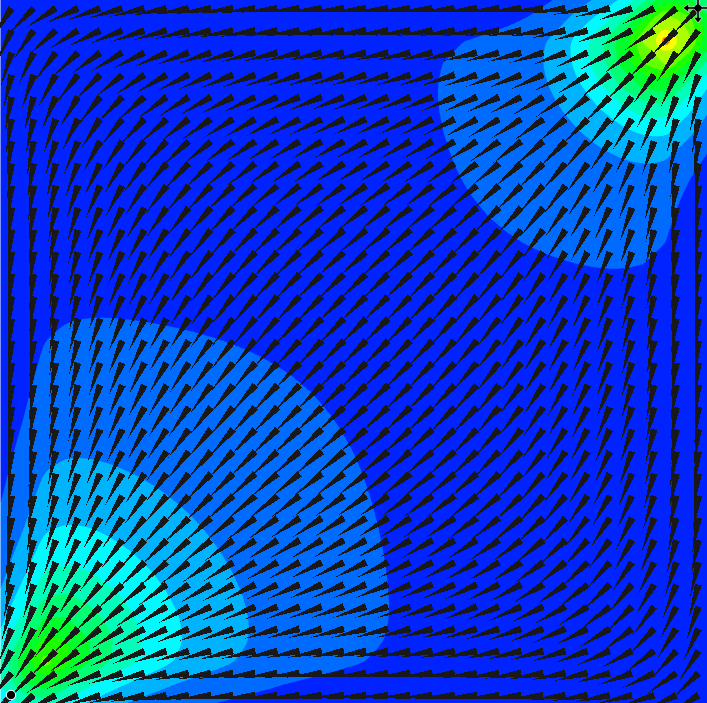
\includegraphics[width=1\linewidth]{displacements.png}
\caption{Карта смещений породы}
\label{displacements}
\end{minipage}
\hfill
\begin{minipage}{0.3\linewidth}
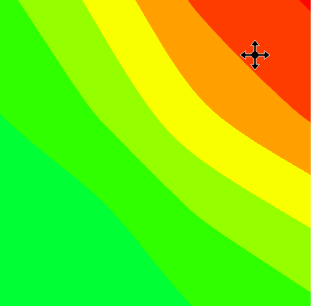
\includegraphics[width=1\linewidth]{injection.png}
\caption{Увеличение порового объема в окрестности нагнетательной скважины}
\label{pore_volume_injection}
\end{minipage}
\hfill
\begin{minipage}{0.3\linewidth}
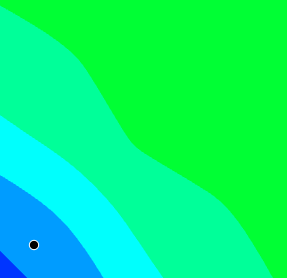
\includegraphics[width=1\linewidth]{production.png}
\caption{Уменьшение порового объема в окрестности добывающей скважины}
\label{pore_volume_production}
\end{minipage}
\end{figure}

\subsection{Учет критерия разрушения породы}
В процессе моделирования разработки месторождения важно учитывать возникновение разрывных нарушений породы. Для учета разрывов материала коллектора используется критерий прочности Мора-Кулона (см. \cite{Belousov}). На рисунке \ref{rock_destruction} показаны нарушения критерия прочности породы в окрестности горизонтальной нагнетательной скважины.

{
\begin{figure}[h!]
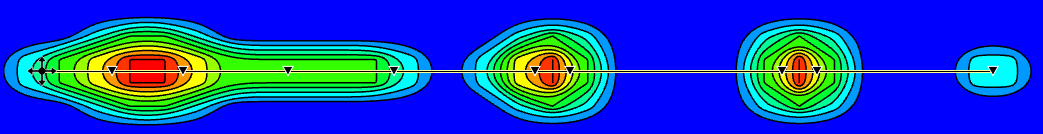
\includegraphics[width=1\linewidth]{rock_destruction.png}
\caption{Карта разрушений породы в окрестности скважины}
\label{rock_destruction}
\end{figure}
}
\section{Выводы}

Предложен метод совместного решения системы уравнений фильтрации вязкой сжимаемой смеси в пористой среде и системы уравнений теории упругости в случае малых деформаций, использующий единую сетку для аппроксимации обеих систем и метод расщепления по физическим процессам для их решения.
Численные эксперименты показали практическую применимость метода.

{
\ifx\undefined\BibEmph\def\BibEmph#1{#1}\else\fi
\ifx\undefined\href\def\href#1#2{#2}\else\fi
\ifx\undefined\url\def\url#1{\texttt{#1}}\else\fi
\ifx\undefined\urlprefix\def\urlprefix{URL: }\else\fi
\ifx\undefined\BibUrl\def\BibUrl#1{\urlprefix\url{#1}}\else\fi
\ifx\undefined\BibUrlDate\long\def\BibUrlDate#1{({%
\cyr\cyrd\cyra\cyrt\cyra\ 
\cyro\cyrb\cyrr\cyra\cyrshch\cyre\cyrn\cyri\cyrya}: #1)}\else\fi
\ifx\undefined\BibAnnote\long\def\BibAnnote#1{#1}\else\fi
\begin{thebibliography}{1}
\addcontentsline{toc}{section}{\bibname}
\def\selectlanguageifdefined#1{
\expandafter\ifx\csname date#1\endcsname\relax
\else\language\csname l@#1\endcsname\fi}

\bibitem{oneway}
\selectlanguageifdefined{english}
\BibEmph{Fredrich J.T.,} One-Way Coupled Reservoir-Geomechanical Modeling of the Lost Hills Oil Field,
\BibEmph{8th U.S. Rock Mechanics Symposium, Washington, DC.}
\newblock 2001.

\bibitem{iterative}
\selectlanguageifdefined{english}
\BibEmph{Settari A., Mourits A.,} Coupled Reservoir and Geomechanical Simulation System,
\BibEmph{SPE J.}
\newblock 2001.
\newblock {\cyr\CYRS.}~219–226.

\bibitem{SPE2015}
\selectlanguageifdefined{russian}
\BibEmph{Богачев К.Ю., Корнева Д.С., Писковский Е.В., Шайбаков А.Л., Эйдинов Д.А.,} Геолого-гидродинамическое моделирование с учетом механических свойств пласта,
\BibEmph{SPE J.}
\newblock 2015.


\bibitem{fully}
\selectlanguageifdefined{english}
\BibEmph{Stone T., Bowen G., Papanastasiou P.,} Fully Coupled Geomechanics in a Commercial Reservoir Simulator,
\BibEmph{SPE J.}
\newblock 2000.

%ЕВП:\bibitem{fullybad}
%ЕВП:\selectlanguageifdefined{english}
%ЕВП:\BibEmph{Chin L.Y., Thomas L.K.,} Fully Coupled Analysis of Improved Oil Recovery by Reservoir Compaction,
%ЕВП:\BibEmph{SPE J.}
%ЕВП:\newblock 1999.

\bibitem{Marchuk}
\selectlanguageifdefined{russian}
\BibEmph{Марчук Г.И.,} Методы вычислительной математики. 
\BibEmph{М.: Наука} 
\newblock 1977.

\bibitem{Aziz}
\selectlanguageifdefined{english}
\BibEmph{Aziz~K., Settari~A.,} Petroleum reservoir simulation.
  \BibEmph{London : Applied Science Publishers}.
\newblock 1979.

\bibitem{Chen}
\selectlanguageifdefined{english}
\BibEmph{Chen Zhangxin, Huan Guanren, Ma Yuanle,} 
Computational Methods for Multiphase Flows in Porous Media (Computational Science and Engineering 2),
  \BibEmph{Society for Industrial and Applied Mathematics, Philadelphia, PA, USA}
\newblock 2006
\newblock {\cyr\CYRT.}~11.
\newblock {\cyr\CYRS.}~193--197.

\bibitem{BogachevMelnichenko}
\selectlanguageifdefined{russian}
\BibEmph{Богачев~К.~Ю., Мельниченко~Н.~С.,} О пространственной аппроксимации
  методом подсеток для задачи фильтрации вязкой сжимаемой жидкости в пористой
  среде, \BibEmph{Вычислительные методы и программирование}.
\newblock 2008.
\newblock {\cyr\CYRT.}~9, {\cyr\textnumero}~2.
\newblock {\cyr\CYRS.}~42--50.

\bibitem{Sedov}
\selectlanguageifdefined{russian}
\BibEmph{Седов Л.И.,} Механика сплошной среды, 
\BibEmph{М.Наука} 
\newblock 1970.
%\newblock {\cyr\CYRS.}~165--170.

\bibitem{Biot}
\selectlanguageifdefined{english}
\BibEmph{Biot M. A.,} General theory of three-dimensional consolidation,
\BibEmph{Journal of Applied Physics, 12}
\newblock 1941.
\newblock {\cyr\CYRS.}~155--164.

\bibitem{Belousov}
\selectlanguageifdefined{russian}
\BibEmph{Белоусов В.В.,} Структурная геология,
\BibEmph{Московский университет}
\newblock 1986.

\end{thebibliography}
}

\end{document}
